\documentclass[letterpaper]{ar-1col}
\usepackage{showyourwork}
\usepackage[letterpaper]{geometry}

\usepackage{natbib}
\usepackage{amsmath}
\usepackage{color}
\usepackage{hyperref}
\usepackage{booktabs}% http://ctan.org/pkg/booktabs
\newcommand{\tabitem}{~~\llap{\textbullet}~~}
%\hypersetup{colorlinks=true,allcolors=[rgb]{0,0,0.8}}

\hypersetup{%
  colorlinks=true,% hyperlinks will be black
  linkcolor=blue,% hyperlink borders will be red
  anchorcolor=blue,
  citecolor=blue,
  menucolor=blue,
  urlcolor=blue,
  pdfborderstyle={/S/U/W 1}% border style will be underline of width 1pt
}


\newcommand{\kms}{km~s$^{-1}$}
\newcommand{\mum}{$\mu$m}

\usepackage{nomencl}
\makenomenclature

\usepackage{graphbox}

\setcounter{secnumdepth}{4}
\usepackage{url}

\usepackage{lipsum}  

% Metadata Information
\jname{Annu. Rev. Astron. Astrophys.}
\jvol{AA}
\jyear{2025}
\doi{10.1146/TBD}

% autoref formatting
\def\sectionautorefname{Section}
\let\subsectionautorefname\sectionautorefname
\let\subsubsectionautorefname\sectionautorefname

% macros
\newcommand{\apjl}{Astrophysical Journal Letters}
\newcommand{\aj}{Astronomical Journal}
\newcommand{\ao}{Applied Optics}
\newcommand{\procspie}{SPIE Proceedings}
\newcommand{\apj}{Astrophysical Journal}
\newcommand{\apjs}{Astrophysical Journal Supplement}
\newcommand{\pasp}{Publications of the Astronomical Society of the Pacific}
\newcommand{\jgr}{Journal of Geophysical Research}
\newcommand{\aap}{Astronomy and Astrophysics}
\newcommand{\mnras}{Monthly Notices of the Royal Astronomical Society}
\newcommand{\actaa}{Acta Astronomica}
\newcommand{\nat}{Nature}
\newcommand{\prl}{Physical Review Letters}
\newcommand{\prd}{Physical Review D}
\newcommand{\ssr}{Space Science Reviews}
\newcommand{\araa}{Annual Review of Astronomy and Astrophysics}

% Symbols
\newcommand{\ydata}{\ensuremath{\boldsymbol{y}}}
\newcommand{\hyperparams}{\ensuremath{\boldsymbol{\phi}}}
\newcommand{\meanparams}{\ensuremath{\boldsymbol{\theta}}}
\newcommand{\dt}{\ensuremath{\tau}}
\newcommand{\amplitude}{\ensuremath{\alpha}}
\newcommand{\lengthscale}{\ensuremath{\lambda}}

\DeclareMathOperator*{\argmax}{arg\,max}

\newcommand{\project}[1]{\textsf{#1}}

% Comments:
\newcommand{\commentehp}[1]{\textcolor{red}{[EHP: #1]}}
\newcommand{\commentmak}[1]{\textcolor{red}{[MAK: #1]}}
\newcommand{\commentsyh}[1]{\textcolor{red}{[SYH: #1]}}

\newcommand{\notebooksuggestion}[1]{\textcolor{blue}{[Notebook: #1]}}

\newcommand{\todo}[1]{\textcolor{red}{[TODO: #1]}}

% message://%3cBYAPR04MB46634305E3091DE92934A5BA8225A@BYAPR04MB4663.namprd04.prod.outlook.com%3e

% Manuscript due date:  September 15, 2024
% Article allotment: 18,000 words, 200 references
% (Estimate the sizes of small figures/tables at 300 words and large ones at 600 words; thus, for every figure/table submitted, please subtract the corresponding number of words from your total allotment. An article length estimator is available online at http://www.annualreviews.org/page/authors/general-information; to access it, select the name of your journal from the drop-down list under Article Preparation and Submission.)  

% Your review article should present a critical appraisal of the significant, rather than the total, literature in the field. This overview may include your own work (even if unpublished). The article should be useful to specialists as well as teachers and scholars from other areas.  It should emphasize where research in a given area should go, as well as where it has been, such that it will influence the future course of knowledge. A list of topics and authors planned for Volume 63 will be sent to you approximately five months before the manuscript due date, and you may wish to correspond with authors whose subjects border on your own.


% Document starts
\begin{document}

% Page header
\markboth{Kenworthy \& others}{HCI}

%TC:ignore

% Title
\title{High Contrast Imaging}

%Authors, affiliations address.
\author{Matthew Kenworthy,$^1$ Sebastiaan Haffert$^2$ and Emiel Por$^3$
  \affil{$^1$Leiden Observatory, Niels Bohrweg 2, Leiden 2300RA, The Netherlands; email: kenworthy@strw.leidenuniv.nl}
  \affil{$^2$Steward Observatory; email: haffert@astronomy.arizona.edu}
  \affil{$^3$STScI; email: epor@stsci.edu}}

%Abstract
\begin{abstract}
High Contrast Imaging will enable the direct detection of photons from rocky terrestrial worlds.
\end{abstract}

%Keywords, etc.
\begin{keywords}
 Optics, coronagraphs, exoplanets, computational methods

\end{keywords}
\maketitle

%Table of Contents
\tableofcontents

\section{INTRODUCTION}
\label{sec:intro}

% High contrast imaging, Lyot corongraph, 2000's development

%TC:endignore

In this review, we provide interactive notebooks that enable the reader to build up their intuition on how coronagraphs work along with wavefront sensing both in the pupil and the focal planes, and how we will tackle the challenges in reaching the contrasts of $10^{-10}$ at angular separations of less than one arcsecond that are required.

% text below from DFM
This manuscript was prepared using the \project{showyourwork} package\footnote{\url{https://show-your.work}} and the source code used to generate each figure is available in a public \project{GitHub} repository\footnote{\url{https://github.com/mkenworthy/ARAA_HCI}}.

To see the specific version of the \project{Jupyter} notebook, that was executed to generate each figure, click on the icon next to the figure caption.

\section{Science Goals}

Initially developed to image the Sun's corona without the need for a Solar eclipse, one of the most significant science drivers for the latest coronagraphs is in the detection and characterisation of circumstellar material and planets around nearby stars.
%
%The scientific goal is to image an exoplanet (a planet orbiting a star other than our Sun) and to characterise its orbit and atmosphere.
%
For an Earth analogue with similar radius, albedo and effective temperature orbiting around a solar-type star 10 parsecs away, the typical amount of reflected light in the optical is $10^{-10}$ of the central star at a separation of 0.1 arcseconds at maximum elongation.
%
The technical challenge is in distinguishing the light of the parent star from the light of the planet.
Planetary systems that are closer to the Sun have two benefits: given two identical planetary systems, one that is twice as close as the other will have twice the angular separation between the star and planet, and from the inverse square law, four times more flux is received from the planet.
%
For direct imaging, therefore, the closest stars to the Sun are the ones that are studied for the presence of directly imaged exoplanets.
%
In a volume limited (20 parsecs) sample of stars around the Sun \citep{2023arXiv231203639K}, there are XXXX solar (G2) type stars, and YYYY M-dwarf stars.
%
DI young Jupiters look are self-luminous in the NIR, but for terrestrial planets, looking for light reflected from the atmosphere/surface, so subject to inverse square law for planet separation from star.


Two regimes: solar analogues at optical wavelengths lead to space based missions, ground based larger aperture telescopes study M dwarf stars that are on average closer to the Sun, and look in the NIR.

Mention HABCAT for a catalogue of solar like stars.

Bioactive molecules see reviews of \citet{2016AsBio..16..465S,2017ARAA..55..433K,2018AsBio..18..663S}.

The search for life beyond the Earth has focused on the idea that water is an essential part of life cycles elsewhere in the Universe, as it is a polar solvent formed from two elements that are found in abundance throughout the Galaxy.
%
Places where water can exist in its liquid state form prime locations for these searches, notably Earth-like planets and ice moons that have a liquid water ocean underneath an ice layer.
%
The region around a star where liquid water can exist on the surface of a terrestrial planet (with appropriate atmospheric pressure) is referred to as the Habitable Zone (HZ); for the Sun this is from 0.9-1.2 au.
%
The HZ changes with stellar evolution as the luminosity of stars changes with time.
%
The angular size of the HZ in diffraction widths can be approximated by XXXXX. 

The nearest stars are taken from the CNS5 \citep{Golovin23}.

This combined with the greater frequency of lower mass stars means that there are two regimes for imaging HZ terrestrial planets around nearby stars: M dwarfs and G-type stars.

For solar type stars, the contrast required in the optical wavelengths is on the order of $10^{-10}$ for terrestrial planets in the HZ of solar type stars, but for smaller mass stars with lower luminosities, the contrast is $10^{-7}$ for M dwarfs since the similar sized planets subtend larger amounts of radiated flux.
%
The markers for biosignatures also set the parameters (such as wavelength and bandwidth) that form part of the design decision.
%
REFS seager, keltenegger, 2018 paper from seager student about false negatives for detecting life, we need multiple signatures. ??? is it this paper? "Molecular simulations for the spectroscopic detection of atmospheric gases" by \citet{Sousa-Silva19}.
%
It is clear that the unambiguous detection of life will require not one singlar detection of a molecule, but will be the combination of several different pieces of evidence.
%
We focus on the technical challenges for imaging a rocky terrestrial planet around a nearby star in our Galaxy.



\begin{figure}[ht]
  \centering
  \script{plot_simple_psf.py}
  \includegraphics[width=1.0\linewidth]{figures/simple_psf.pdf}
  \caption{Figure run from a static Python script.}
  \label{fig:simplepsf}
\end{figure}



% \begin{figure}[ht]
%   \centering
%   \script{interactive_fresnel.ipynb}
%   \includegraphics[width=1.0\linewidth]{figures/test.pdf}
%   \caption{Figure run from a Jupyter notebook.}
%   \label{fig:fresnel}
% \end{figure}


\begin{armarginnote}[]
  \entry{HCI}{High Contrast Imaging}
  \entry{FP}{Focal Plane}
  \entry{PP}{Pupil Plane}
  \entry{FPWFS}{Focal Plane Wavefront Sensing}
  \entry{WFS}{Wavefront Sensor}
\end{armarginnote}


\section{From Maxwell's Equations to Wavefronts}
The vast majority of energy from astrophysical objects arrives at our telescopes in the form of electromagnetic radiation.
%
%The electromagnetic waves propagate through space by exchanges between the electric and magnetic fields because a changing electric field induces a magnetic field and vice-versa.
%
This time-dependent interaction is described by Maxwell's equations,

\begin{equation}
\begin{aligned}
\frac{\partial\mathcal{D}}{\partial t} \quad & = \quad \nabla\times\mathcal{H},   & \quad \text{(Faraday's law)} \\[5pt]
\frac{\partial\mathcal{B}}{\partial t} \quad & = \quad -\nabla\times\mathcal{E},  & \quad \text{(Ampere's Law)}   \\[5pt]
\nabla\cdot\mathcal{B}                 \quad & = \quad 0,                         & \quad \text{(Gauss's law)}   \\[5pt]
\nabla\cdot\mathcal{D}                 \quad & = \quad 0.                         & \quad \text{(Coulomb's law)}
\end{aligned}
\end{equation}
This form of Maxwell's equations is in the material form without any charge and current sources. The material form is used to describe the propagation of electromagnetic fields inside matter. This set of equations is completed by describing the particular matter of the medium with the constitutive relations, $D=\epsilon E$ and $B=\mu H$. Here $\epsilon$ and $\mu$ are the permittivity and magnetic permeability, respectively. The wave equation for electromagnetic waves can be derived by taking the curl of Ampere's law. This gives us the classic wave equation if we assume that the EM wave propagates in isotropic and homogeneous materials,
\begin{equation}
\label{eq:wave_eq}
\begin{aligned}
%\nabla\times\frac{\partial\mathcal{B}}{\partial t} \quad  =& \quad -\nabla\times\nabla\times\mathcal{E} \\
%\frac{\partial\nabla\times\mathcal{B}}{\partial t} \quad  =& \quad -\nabla^2\mathcal{E} \\
%\frac{\partial\nabla\times\mathcal{\mu H}}{\partial t} \quad  =& \quad -\nabla^2\mathcal{E} \\
%\mu\frac{\partial^2 \mathcal{D}}{\partial t^2} \quad  =& \quad -\nabla^2\mathcal{E} \\
\mu \epsilon \frac{\partial^2 \mathcal{E}}{\partial t^2} - \nabla^2\mathcal{E} = 0 .
\end{aligned}
\end{equation}
Let's now consider a purely monochromatic EM wave with frequency $\omega$. The wave function is then $\mathcal{E}=\psi(r) e^{iwt}$ with $\psi(r)$ describing the spatial distribution. Substituting this relation into Equation \ref{eq:wave_eq},
\begin{equation}
\nabla^2\mathcal{E} +\mu \epsilon \omega^2 \mathcal{E} = 0.
\end{equation}
The usual definition of the permittivity and permeability are $\epsilon=\epsilon_r \epsilon_0$ and $\mu=\mu_r \mu_0$ with $\epsilon_r$ and $\mu_r$ the relative permittivity and permeability compared to that of vacuum, $\epsilon_0$ and $\mu_0$. In optics most glasses and materials are defined by their refractive index $n$ which is related to permittivity as $\epsilon_r = n^2$ and many of these are also non-magnetic which means that $\mu_r=1$. Substituting this will give us the classic Helmholtz equation
\begin{equation}
\nabla^2\mathcal{E} + n^2k^2 \mathcal{E} = 0,
\end{equation}
We made use of the fact that the speed of light is $c = \frac{1}{\sqrt{\epsilon_0\mu_0}}$ and that $k = c\omega$ is the wave number. The propagation through an optical system has a preferential direction that is usually defined along the z-axis. The z-axis evolution can be derived by separating the spatial components into the z component and the perpendicular components (x,y),
\begin{equation}
\frac{\partial^2\mathcal{E}}{\partial z^2} = -\nabla_{\perp}^2\mathcal{E}-n^2k^2 \mathcal{E},
\end{equation}
This differential equation can be solved by assuming a plane wave expansion $\mathcal{E}(x,y,z)=e^{i(k_x x + k_y y)}f(z)$ which results in
\begin{equation}
\frac{\partial^2\mathcal{E}}{\partial z^2} = -(n^2k^2 - k_{\perp}^2)\mathcal{E}.
\end{equation}
The solution to this equation is the so called Angular Spectrum Propagator that relates the electric field at any one plane to the electric field at any other,
\begin{equation}
\label{eq:angular_spectrum}
\mathcal{E}(x, y, z') = \mathcal{F}_{x,y}^{-1}\{e^{-ik_z(z'-z)}\mathcal{F}_{x,y}\{\mathcal{E}(x,y,z)\}\}.
\end{equation}

Here the z component of the wave vector is defined as $k_z=\sqrt{n^2k^2 - k_{\perp}^2}$ and $\mathcal{F}_{x,y}^{(-1)}$ is defined as the (inverse) Fourier transform over the x and y coordinates. While Equation \ref{eq:angular_spectrum} describes the full propagation from one plane to another, it is quite unwieldy to use and does not provide much physical insight. For many optical systems it is sufficient to analyze the paraxial performance. The paraxial approximation assumes that the plane waves make small angles with respect to the z-axis which means that the x and y wave vector components are $k_x,k_y<<1$. In this regime the propagation factor $k_z=\sqrt{n^2k^2 - k_{\perp}^2}\approx nk - \frac{k_{\perp}^2}{2nk}$
\begin{equation}
\label{eq:angular_spectrum2}
\mathcal{E}(x, y, z') = e^{-ink(z'-z)} \mathcal{F}_{x,y}^{-1}\{\mathcal{F}_{x,y}\{\mathcal{E}(x,y,z)\}\}.
\end{equation}
%$$E(\mathbf{r},t)=E_0(\mathbf{r})e^{i(\mathbf{k}.\mathbf{r}-\omega t)}$$

%Maxwell's equations describe the time-dependent interaction between static and moving electric charges, electric fields and magnetic fields.


%When a star is imaged with a large ground based telescope the detector does not see a point source with all flux concentrated into one pixel, but instead the stellar flux is distributed across a finite area.%actually an infinite area because band-limited signals have an infinite support. There is no end to the Airy pattern.

%
%This is due to the wave-like nature of electromagnetic radiation.


% ENERGY PROPAGATION
%Energy is stored in both the electric and magnetic fields.
% WAVE SOLUTIONS
%One solution to these equations are second-order differential wave equations, which describe a periodic change in the electric and magnetic field strength throughout a given volume.
%
%In the absence of any free electrical charges, these show that, energy is propagated in a direction along their direction of motion. BLAH NOT TRUE FOR CALCITE...
% ENERGY IN E FIELDS
%The majority of energy is stored in the electric field, and since the magnetic field strength follows the electric field strength we only talk about the time and space evolution of the electric field.

%The time-varying electric field strength of an electromagnetic plane wave at time $t$ is described by:

%$$E(\mathbf{r},t)=E_0(\mathbf{r})e^{i(\mathbf{k}.\mathbf{r}-\omega t)}$$
%where $\mathbf{r}$ is a point in three-dimensional space, $\mathbf{k}$ is a unit vector pointing in the direction of the wave propagation, and $\omega$ is the angular frequency of the wave.
%
%The angular frequency and wavelength of the wave is related by $\omega = 2\pi c/\lambda$ where $c$ is the propagation speed in free space.
%
% PHASE only applies to a periodic wave!

%Waves are periodic functions, so we introduce the concept of phase: the distance (in space or time) from a reference point in the amplitude of wave, usually defined so that a phase of zero is the place/time where the amplitude of the field is the largest. UGH NOT QUITE RIGHT. 

%A wavefront is a surface with constant phase.
%
%For an electromagnetic wave propagating through free space, it is a flat two dimensional plane.
%
%This plane moves in the direction of propagation $k$.

%Optical elements bring separate spatial regions of the wave to the same spatial point.
%
%Since the wave is coherent, the resultant electric field is a linear addition of the electric field propagated along the optical path length difference.
% Maxwell's equations are linear and so superposition of different k vectors and different omegas are possible
%
% The wave propagation has k = E x B, so all three quantities are perpendicular to each other.

%There are two orthogonal solutions, corresponding to two independent polarizations for electromagnetic waves.

%Ultimately, if we know the electric field distribution at the telescope aperture then we can propagate the resultant electromagnetic waves through our telescope and instrument to subsequent focal and pupil planes.

The coherent superposition of electric fields from different parts of the telescope aperture and the associated phase offset gives rise to \textbf{interference}, where the sum of all these electric amplitudes can give very different results from an incoherent addition of the fluxes.

\section{Definition of quantities}

\nomenclature{$i$}{The imaginary unit}

\nomenclature{$c$}{Speed of light in a vacuum}
\nomenclature{$\vec{E}$}{Electric field}
\nomenclature{$\vec{H}$}{Magnetic field}
\nomenclature{$\mathcal{D}$}{Displacement field}
\nomenclature{$\mathcal{B}$}{Magnetizing field}
\nomenclature{$\epsilon$}{Electric permittivity}
\nomenclature{$\epsilon_0$}{Electric permittivity of vacuum}
\nomenclature{$\mu$}{Magnetic permittivity}
\nomenclature{$\mu_0$}{Magnetic permittivity of vacuum}
\nomenclature{$\omega$}{Wavenumber}
\nomenclature{$\vec{k}$}{Wavevector}

\nomenclature{$\lambda$}{Wavelength}
\nomenclature{$\lambda_0$}{Center wavelength in the bandpass}
%\nomenclature{$\delta\lambda$}{d}
\nomenclature{$\Delta\lambda$}{The width of the bandpass}

\nomenclature{$D$}{Diameter of the pupil}

\nomenclature{$n$}{(Complex) refractive index of a macroscopic material}
\nomenclature{$\mathcal{F}_{x,y}[\cdot]$}{Fourier transform operator}
\nomenclature{$\mathcal{F}^{-1}_{x,y}[\cdot]$}{Inverse Fourier transform operator}
\nomenclature{$C_\lambda[\cdot]$}{A general coronagraph propagation operator}

\nomenclature{$\Psi_\lambda[\vec{k}]$}{Coronagraphic image}
\nomenclature{$\phi$}{The phase of the electric field}
\nomenclature{$\alpha$}{The amplitude of the electric field}
\nomenclature{$\Pi$}{The telescope pupil function.}

\printnomenclature

\section{Diffraction of simple apertures}
\notebooksuggestion{different apertures and geometries}

A square aperture with a side length of $D$ illuminated by light of wavelength $\lambda$ will produce the illumination seen in Figure XXXX.
%
The focal plane is divided by a rectilinear dark grid
%
The angular distance from the optical axis to the first dark minimum is $\lambda/D$ in units of radians.

For a circular unobstructed telescope aperture, this pattern is referred to as the Airy function.

\section{The Lyot Coronagraph}

\notebooksuggestion{lyot fully adjustable}
Stellar coronagraphs have now been in use for several decades. However, the first coronagraph was developed by Bernard Lyot to observe the corona of the Sun in the 1930s. It took over half a century before astronomers applied coronagraphs to image the faint cirumstellar environment by blocking starlight. 

The first coronagraph to successfully image a debris disk was a Lyot coronagraph built by \citet{Vilas87} and it imaged the edge-on circumstellar disk around Beta Pictoris in 1984 \citep{Smith84}.
%
The optical layout of the Lyot coronagraph can be generalised in Figure XXXXX, with the letters A-F representing the images present at that location in the coronagraph light path.
%
The telescope pupil (A) is reimaged into a focal plane of the sky (B) where an opaque mask that has high absorptivity and low reflectivity blocks the light from any on-axis source (C).
%
Optics then form an image of the resultant pupil (D) to an intermediate pupil plane, where a second opaque mask - the Lyot stop - is located.
%
This Lyot stop blocks the diffracted light of the star - now forming a ring of light along the outer edge of the telescope pupil (E).
%
A second optical system then reimages the resultant focal plane of the instrument onto a detector (F).
%
%When an object is placed behind the focal plane mask, the light from that object is blocked and does not go any further.
%
Any circumstellar objects outside the radius of the focal plane mask then pass through unimpeded through the coronagraph and are subsequently reimaged in the detector focal plane at F.
%
The light rays pass through the coronagraph optics to form an image at F with only minor modification: the reimaged pupil at D is superficially very similar to the telescope pupil A.

For an on-axis source, the removal of the Airy core plus attendant diffraction rings significantly modifies the wavefront passing through the coronagraph, resulting in a flux redistribution at D where the flux is concentrated in a ring whose peak brightness lies along the perimeter of the reimaged telescope pupil, extending both beyond the radius of the pupil and into the centre of the pupil.

The purpose of the Lyot stop is to remove as much of this ring of light as possible, whilst maximising the throughput of the pupil image D for off-axis sources.
%
Adjusting the diameter of the focal plane mask changes the full width half maximum of the ring of light at D, which requires a smaller Lyot stop to block - but then the throughput of the pupil for off-axis sources then decreases.
%
Decreasing the Lyot stop aperture has a second impact in that the reduced pupil diameter increases the Full Width Half Maximum (FWHM) of the images in the final focal plane F, spreading the flux from the off-axis sources over a larger area in the detector and degrading the angular resolution of the telescope and instrument.
%
The optimal diameters of the Focal Plane Mask (FPM) and Lyot stop aperture are then driven by the science requirements - how close to the central star (measured in diffraction widths at the lower spatial resolution) should the coronagraph be able to transmit light from off-axis objects in the field of view.

\section{Beyond Lyot with complex pupil and focal plane masks}

The Lyot coronagraph was designed at the time when it was still difficult to precisely manipulate the phase of light with optics.
%
With the advent of more advanced manufacturing capabilities, very precise phase control became possible.
%
This was a significant boost to the design toolbox for coronagraphs.
%
The major downside of the classic Lyot coronagraph is that only the light that falls on the opaque FPM gets blocked.
%
Any light that is off-axis will pass through the system.
%
This holds not only for light that comes from off-axis sources but also for aberrations that causes light to end up outside of the FPM.
%
A bigger mask will be able to block a larger fraction of the light and therefore achieve a deeper contrast.
%
However, if the mask is made larger the inner-working angle also becomes bigger and that means fewer planets will be accessible.
%
A smaller inner-working angle is crucial both for the extremely large ground-based telescopes and the space-based telescopes. 

\subsection{Focal plane phase mask coronagraphs}

Focal plane phase masks offer a solution.
%
Phase masks don't enhance the contrast by blocking light but by phase shifting a part of the PSF (usually the core of the PSF).
%
The phase shifted part then causes destructive interference at the Lyot plane.
%
The Lyot stop blocks the areas where the light does not destructively interfere.
%
The 50\% encircled energy radius is on the order of $\sim \lambda/D$ for almost all aperture shapes.
%
This means that it is possible to achieve perfect destructive interference with a mask that has a size on the order of $\lambda/D$.
%
This is the central idea that was used to design the Roddier and Roddier (RR) phase mask \cite{roddier1997stellar}.
%
The RR mask covers the core of the Airy pattern that contains 50\% of the encircled energy and phase shifts the core by $\pi$ to cause destructive interference.
%
The RR mask works well for monochromatic light, but over broad spectral bandwidths it degrades in contrast
%
Diffraction causes wavelength scaling of the PSF that either makes the focal plane mask too big or too small compared to the PSF.
%
Masks made out of multiple concentric rings, such as the dual-zone phase mask \citep{soummer2003achromatic}, were proposed to increase the spectral bandwidth.

Further achromatization for larger spectral bandwidths is possible by designing inherently achromatic phase masks.
%
Inherent achromatic masks are scale invariant, which means that they always look the same regardless of the size of the PSF.
%
One of the most used phase mask coronagraphs is the vortex coronagraph (VC).
%
The VC uses a phase mask with a vortex pattern where the phase changes with the azimutal angle: $\phi=q \cdot \theta$ with $q$ the charge, i.e. the number of times the phase wraps around, of the vortex and $\theta$ the azimuth angle.
%
Another example is the Four Quadrant Phase Mask (FQPM).
%
The FQPM splits the focal plane in four quadrants and applies a checkerboard phase pattern.
%
The scale invariant phase masks of these two coronagraphs are shown in Figure \ref{fig:scale_invariant}.

\begin{figure}[ht]
  \centering
  \script{plot_scale_invariant_masks.py}
  \includegraphics[width=0.5\linewidth]{figures/scale_invariant_masks.pdf}
  \caption{The focal plane phase functions of two scale invariant coronagraphs.
  %
  The left figure shows the four quadrant phase mask and the right figure shows the optical vortex phase mask.}
  \label{fig:scale_invariant}
\end{figure}

Both phase masks that are shown in Figure~\ref{fig:scale_invariant} completely null out all on-axis light from a clear aperture.
%
This property is why both the FQPM and the OVC have been extensively studied over the past several decades.
%
The inner-working angle of both coronagraph approaches 1 $\lambda/D$ which makes coronagraphy possible at the diffraction limit!
%
The Four Quadrant Phase Mask (FQPM) was implemented on SPHERE \citep{Boccaletti04} and is currently the coronagraph on JWST with the smallest inner-working angle and has been recently used to characterize a planet at 1.8 $\lambda/D$ \citep{franson2024jwst}. 
 
%All ground-based telescopes need to image through Earth's atmosphere. The turbulent nature of the atmosphere causes aberrations that degrade the imaging qualities of the telescope. In such conditions, it is very difficult to optimally reject starlight because what electric field actually needs to be rejected? Is it the electric field that is measured now, or the differently aberrated electric field 20 milliseconds from now? The constantly changing electric field of the incoming light made it difficult to create more advanced coronagraphs. The classic Lyot coronagraph design was not improved upon until the advent of large aperture telescopes with adaptive optics systems that had a high enough performance to deliver diffraction-limited images.
%
%These telescopes made the imaging of low mass substellar companions (brown dwarfs and young self-luminous planets) feasible for the first time.

%
%After the discovery of Gliese 229B (XXX CHECK WAS THIS A LYOT?) with the Palomar 5m PALM 5000 system, a series of coronagraphic designs appeared where researchers explored the different possibilities of placing complex amplitude apodizers at both the focal plane and pupil plane locations.
%
%A wide range of coronagraph designs were explored, including XXXXX focal plane, pupil plane, telephone list of all different coronagraphs.
%
%MENTION interferometer concepts.


%FINISH 2 SENTENCES SH 



\begin{table}
  \centering
  \begin{tabular}{lll}
    \toprule
    \multicolumn{3}{c}{Comparison of PPM and FPM coronagraphs} \\[.5\normalbaselineskip]
     & Focal Plane Masks & Pupil Plane Masks \\
    \midrule
    Advantages \\
     & \tabitem Small IWA & \tabitem Pointing invariant \\
     & \tabitem High transmission & \tabitem Single optic \\
     & \tabitem 360 deg FOV & \tabitem Any telescope mirror geometry \\
    Disadvantages \\
     & \tabitem Stellar leakage & \tabitem Complex manufacture \\
     & \tabitem Pointing sensitive & \tabitem Larger IWA \\
     & \tabitem Complex deisgn with tel pupils & \tabitem Lower planet throughput \\
     & \tabitem Lyot stop required & \tabitem Smaller FOV \\[.5\normalbaselineskip]
    \bottomrule
  \end{tabular}
\end{table}


\subsection{Pupil plane mask coronagraphs}

All stars have a small but finite angular diameter on the sky, typically $\lambda/100$ or less but $\lambda/10$ is possible for the closest stars.
%R
In the visible, median stars for HWO are going to be $\lambda/10$, with some a little larger, becoming even larger as the apertures for ELTs will be larger by a factor of a few: Proxima Centaurihas a diameter of 1 mas, which is 1/3 to 1/6 $\lambda/D$ for ELT and GMT.
%
The disk of the star can be treated as a set of incoherent point sources, and so the small but finite angular size of the star means that the sensitivity of contrast of focal plane coronagraphs varies as a function of angle.
%
Given that the star is tens of thousands to millions of times brighter than the target planet, even a small amount of stellar leakage can overwhelm the flux from the planet.

Apodizing the telescope pupil provides an opportunity to redistribute the light in the science camera focal plane to form `dark zones' around the target star where an exoplanet can be imaged.
%
Strictly this is not so much a coronagraph as a modification to the PSF of the instrument - all objects in the focal plane have the same PSF, both stars and exoplanets together.
%
As long as the angular diameter of the star is smaller than the Airy core of the PSF, pupil plane coronagraphs are not impacted by the diameter of the star or by residual tip tilt vibrations that are not removed by the Adaptive Optics control loop, making them a robust alternative to the more efficient, smaller IWA focal plane coronagraphs. 
%
Suppressing diffraction in the PSF requires destructive interference using coherent light from the Airy core, but at a cost in Strehl ratio of the PSF.
%
Since the exoplanet PSF is identical to the stellar PSF, the planet throughput decreases too.



\section{Parameters to optimize}

As the previous section explained, clear apertures have solutions that perfectly remove any on-axis light. However, real systems are not ideal and generally don't have a clear aperture. Even more important, stars are not ideal point sources. Solutions that only work for point sources are already out of the question then. The current and future generation of coronagraphs are designed to take on non-ideal environments. This means that the coronagraph is optimized for a specific list of parameters during the design process.

The first set of parameters are the inner-working angle (IWA) and the outer-working angle (OWA). The IWA is usually set to the angular separation where the throughput is 50\% of the peak off-axis throughput. The IWA and OWA set the smallest and largest angular separation of the dark hole region that the coronagraph will make. Some coronagraphs, such as the OVC or FQPM, don't have an OWA only an IWA. Figure \ref{fig:coronagraph_focal_plane_definitions} shows a coronagraphic dark hole with the definition of the IWA and OWA.

\begin{figure}[ht]
  \centering
  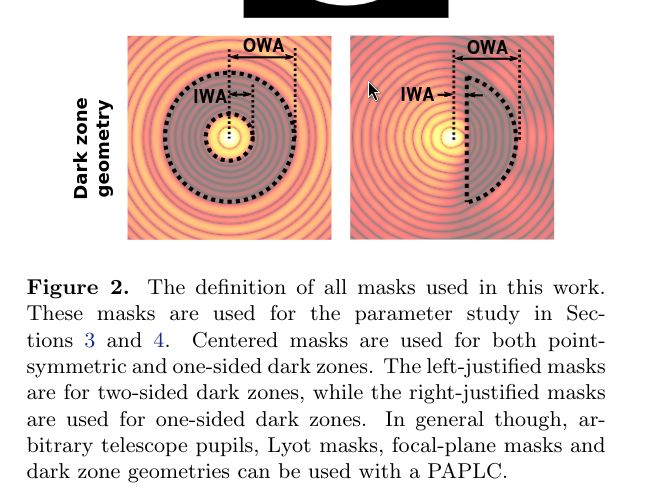
\includegraphics[width=0.5\linewidth]{figures/dark_hole_definition.png}
  \caption{ADD caption \textcolor{red}{TODO: replace with our figure instead of Emiel's}}
  \label{fig:coronagraph_focal_plane_definitions}
\end{figure}

The contrast and throughput are the next set of parameters that we need to optimize for.
%
The contrast sets the amount of starlight that is left after the coronagraph. It is important to define the term contrast as this can mean many different things.
%
\citet{ruane2018review} provide a thorough overview of the different metrics and their definition.
%
The contrast is defined as
\begin{equation}
C = \frac{\eta_*(\vec{r})}{\eta_p(\vec{r})}.
\end{equation}
Here $\eta_*(\vec{r})$ is the fractional throughput of the star at focal plane position $\vec{r}$ integrated over a photometric aperture.
%
This is then divided by $\eta_p(\vec{r})$ the fractional throughput of the planet in the same photometric aperture.
%
This normalizes the contrast w.r.t. the throughput of the planet, which is important because the planet throughput usually varies as function of angular separation. %
%
Both the contrast $C$ and $\eta_p(\vec{r})$ need to be included in the optimization process.
%
The first to make sure that the starlight is nulled and the second to make sure that the planet light is maintained.
%
This optimization has to be done over a certain spectral bandwidth $\Delta \lambda$.

The corongraphs that are designed with only the previous set of optimization targets are not optimal in real environments.
%
In real instrument environments there are wavefront aberrations and small instrumental drifts.
%
These cause light to leak around the coronagraph and cause residual stellar speckles.
%
The coronagraphs must be made robust against low-order wavefront errors and other instrumental drifts.
%
Other more practical things to consider are the precision with which we can align an instrument. %
%
For example, how well can the Lyot stop be aligned?
%
The performance of a coronagraph might be extremely sensitive to the Lyot stop alignment, which means that theoretically the coronagraph delivers the contrast but practically it will never reach it.
%
Therefore, alignment tolerancing must be included in the coronagraph design to make sure the target performance is achieved.

In this way, there are many other nuisance parameters that can be included.
%
However, the numerical optimization will take significantly longer if more parameters are included.
%
A good coronagraph designer will therefore make a trade-off between which parameters are required, good to have and not significant.

\section{Wavefront Sensing and Correction}

The coronagraph designs assume that the incoming wavefronts from all the astrophysical sources in the field of view are flat, and that the optics in the coronagraph are ideal, propagating and modifying these wavefronts without distortion to the final science camera focal plane.
%
In reality, however, there are several factors that cause deviations of the wavefronts from this ideal: (i) optical manufacturing limitations, (ii) environmental conditions (both static and dynamic) within the instrument and the telescope, and in the case of ground based telescopes, (iii) the wavefront residuals from the Earth's turbulent atmosphere partially corrected with a high order adaptive optics system.

\begin{armarginnote}[]
  \entry{DM}{Deformable Mirror}
  \entry{FPM}{Focal Plane Mask}
  \entry{PP}{Pupil Plane Mask}
  \entry{WFS}{Wavefront Sensor}
  \entry{AO}{Adaptive Optics}
\end{armarginnote}

\subsection{Adaptive Optics}

Adaptive optics sense the turbulence introduced by the Earth's atmosphere using Wavefront Sensors, reconstruct an estimate of this turbulence, and use an electronically actuated deformable optical element - typically a Deformable Mirror (DM)\footnote{There are several other optomechanical devices that exploit other optically active principles to modify a wavefront.}) - within the instrument to modify the incoming turbulent wavefront and flatten it.
%
With the DM upstream of the WFS, and a control computer providing the calculation of wavefront measured by the WFS and applying this correction to the DM, this forms a {\bf closed loop}, where the response of the DM's correction is seen by the WFS in the instrument.

The Earth's atmosphere is highly dynamic and changes on a timescale of milliseconds, but the wavefront reconstruction and correction on the DM is not instantaneous, leading to a small but significant time lag between measurement and the application of the correction.
%
Adaptive optics is a complex and mature field in its own right, covering atmospheric turbulence, optomechanics, engineering control theory, wavefront sensing and information theory (each of these topics would be a review in their own right), but for now we refer the reader to XXX and YYY for reviews on these topics. 
%
For our purpose, we assume that ground based instruments have a high order adaptive optics system providing high order wavefront correction, resulting in a time evolving screen of residual phase errors that change on a timescale of milliseconds and have $\lambda/20$ r.m.s.

\subsection{Non-common path aberrations}

Aberrations can be sensed and corrected to the point of the last wavefront sensor in the optical path other high contrast instrument.
%
Many AO systems take advantage of the fact that the optical path difference (OPD) introduced by the Earth's atmopshere above groud based telescopes is achromatic, despite this OPD
 
{\bf TODO MAK}


The conceptual design of GMagAO-X by \citet{Males22}.

Lives of speckles by \citet{Males21}.

%Jared's AO4 ELT paper was a good talk, but this is the argument to limit to 30 parsec.

Fundamental sensitivity limite on apertures with PIAA-ZWFS on \citet{Haffert23}

Haffert 2023 talk mentioned this ore we can talk about it below:

%Diffraction limit of telescope is almost fundamental limit. The HZ stays fixed in linear space, but the angular size shrinks with distance of star from Sun.

Apparent magnitude of the stars goes down, AO performance goes down, halo fills in.

Extreme Adaptive Optics ARAA in \citet{Guyon18}

Guoyn 2005 fundamental WFS in \citet{Guyon05-1}

Jared and Guyon 2018/19 on predictive control and speckle lifetime - \citep{Males18}


Jared 2020 speckle lifetime \citep{Males21}

self coherent camera (Pierre? Baudoz 2006 original \citep{Baudoz06}) refael Galicher paper from 2010 instead/as well Self-coherent camera as a focal plane wavefront sensor: simul \citep{Galicher10}.




2022 on sky EFC axel potier \citep{Potier22} and the first paper in the series on VLT/SPHERE is \citep{Potier20} and on sky efc with FQPhase Mask to demo on-sky EFC is paper III and is \citet{Galicher24}.




\section{ELTs for M dwarf exoplanets}

{\bf TODO MAK}

Guyon has a nice figure... 2014 or 2016 SPIE proceeding. Maybe Emiel's phd thesis introduction on this.

Cite papers about METIS \citep{Brandl21} has high contrast imaging modes \citep{Kenworthy16,Carlomagno20}.

PCS roadmap paper \citep{Kasper21}

GMagAOX from Jared Males 2022/2024 \citep{Males22}.

TMT papers on the PSI \citet{Jensen-Clem22,Fitzgerald22}


XXX put an approximate outer limit on the distance for direct imaging. HZ of solar star is 

$DL_{HZ} = 1/$

\notebooksuggestion{play with different contrasts and IWA to see yields}

%\lipsum[2]

\section{Space coronagraphs and HWO for G type stars}

Chris Stark Space telescope yield papers...\citep{Stark14,Stark24}.

\lipsum[2-4]



\section{Polarization effects} 
%van Holstein 2023 paper \citep{vanHolstein23} and \citep{vanHolstein20}.
%SPHERE in 202x on beam shifts zimpol \citep{Schmid18}.
%polarization in the PSF: \citep{Breckinridge15}
%Chipman 1989 Polarization analysis of optical systems. \citep{Chipman89}
%Polarization aberrations in next-generation giant segmented mirror telescopes (GSMTs). I. Effect on the coronagraphic performance: \citet{Anche23}

\notebooksuggestion{Polarimetric beam shift using Fresnel equation - Change angle of incidence and show differential beam shift.}

The field of high-contrast imaging is always hammering away at one noise floor after another. It started with the common phase aberrations that dominate at low to moderate contrast. After that, amplitude aberrations started to limit the contrast. This was solved by using multiple deformable mirrors. Now, the contrasts that are achieved on-sky and on testbeds reveal another limit; polarization. Polarization is an often underappreciated property of light. The derivation shown in Section \ref{sec:maxwell} actually also ignores the effects of polarization which was done for mathematical clarity. However, light consists of two orthogonal polarizations states that do not interfere with each other. That means that there are, at any time, always two beams of light propagating through our coronagraph that might interact in a different way with the instrument. A more detailed treatment of polarization and physical optics propagation can be found in the literature \citep{McLeod14}.

The Fresnel equations describe how light is either reflected off or transmitted through an interface. The equations also show that different polarization states have different Fresnel coefficients. This wouldn't be a problem if the Fresnel equations did not also depend on the angle of incidence. The definition of all variables for the incidence, reflected and transmitted wave are shown in Figure \ref{fig:fresnel_equations}.

The Frensel equations for plane wave interfaces are,
\begin{align}
r_s = \frac{n_1\cos{\theta_i} - n_2\cos{\theta_t}}{n_1\cos{\theta_i} + n_2\cos{\theta_t}},\\
t_s = \frac{2n_1 \cos{\theta_i}}{n_1\cos{\theta_i} + n_2\cos{\theta_t}},\\
r_p = \frac{n_2\cos{\theta_i} - n_1\cos{\theta_t}}{n_2\cos{\theta_i} + n_1\cos{\theta_t}},\\
t_p = \frac{2n_1 \cos{\theta_i}}{n_2\cos{\theta_i} + n_1\cos{\theta_t}}
\end{align}

\begin{figure}[ht]
  \centering
  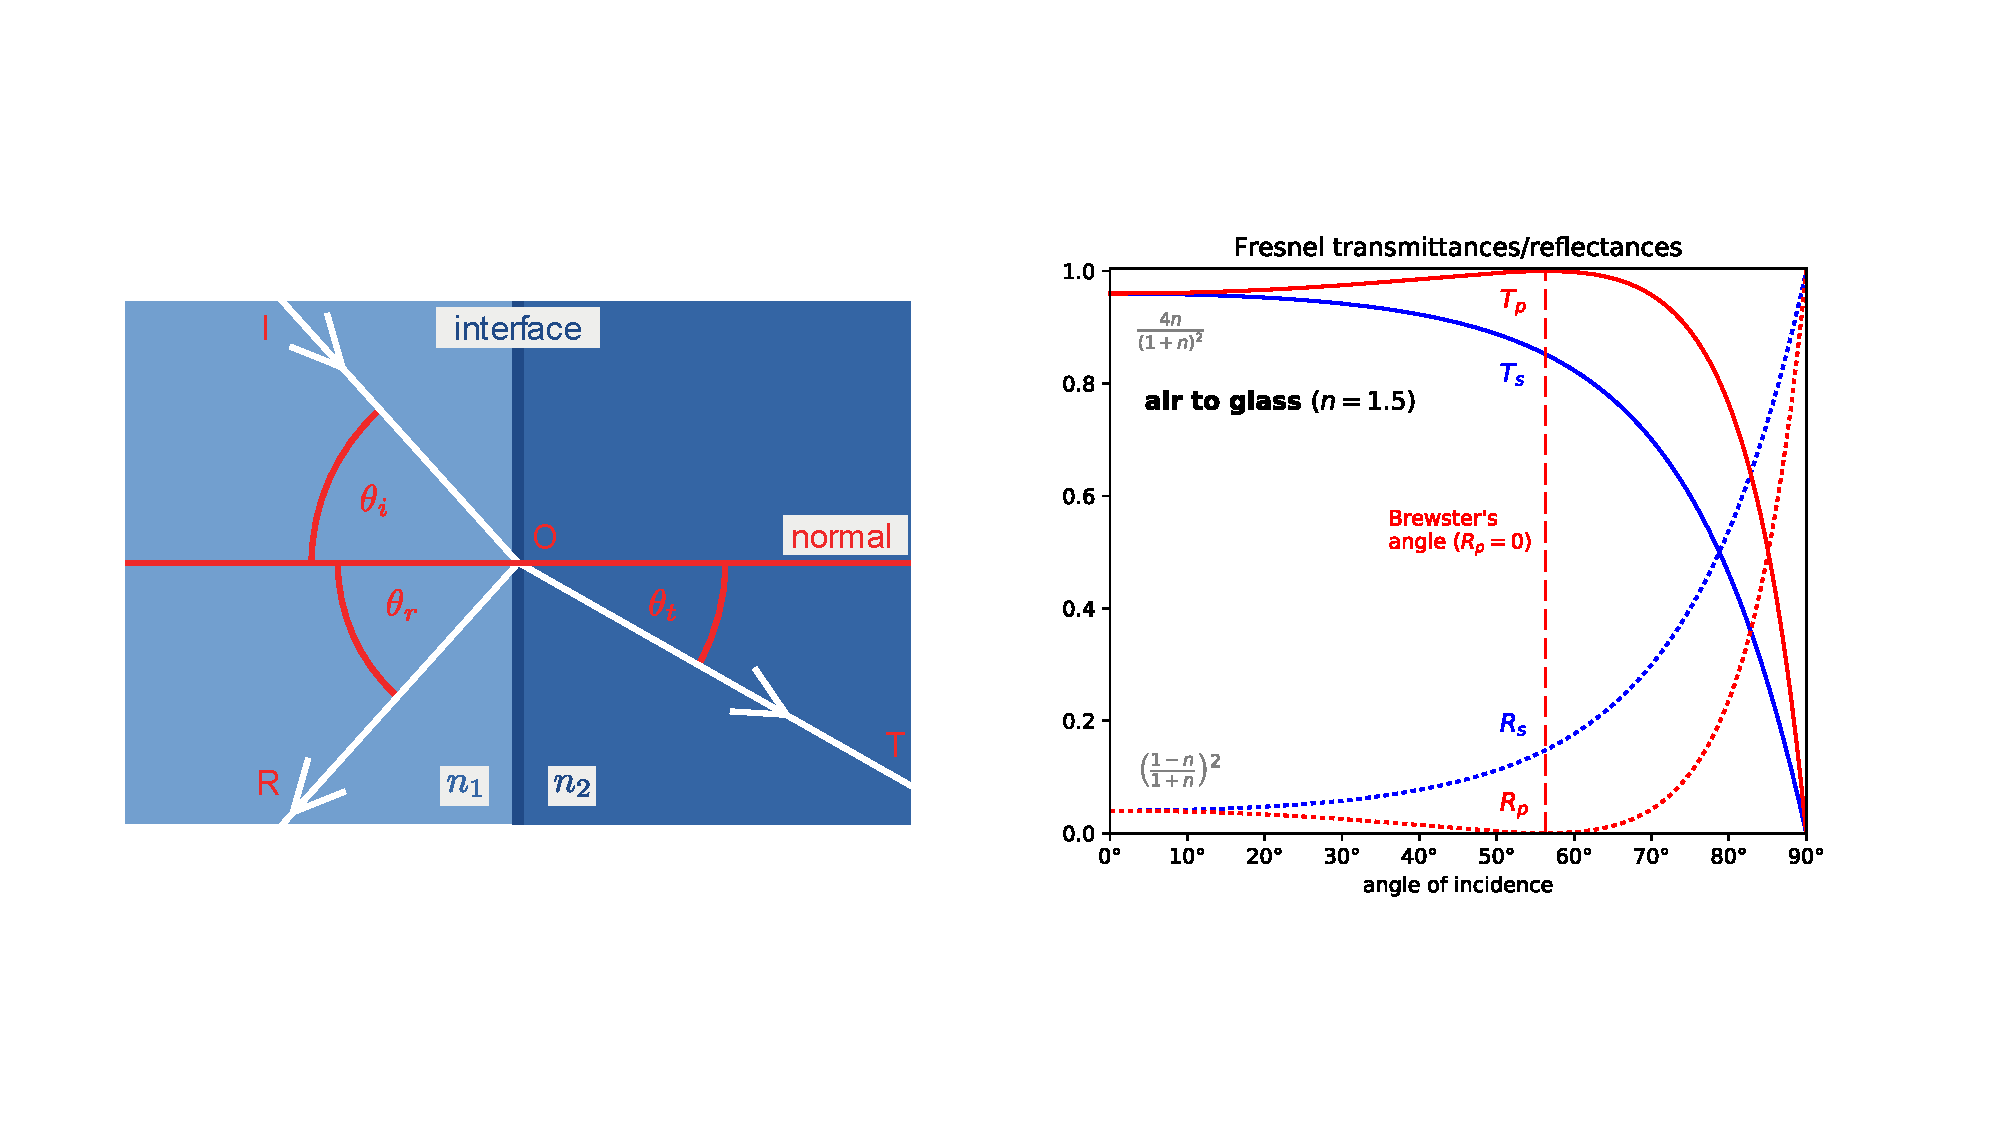
\includegraphics[width=\linewidth]{figures/fresnel_equations_figure.pdf}
  \caption{}
  \label{fig:fresnel_equations}
\end{figure}

\section{PIAA}\label{sec:piaa}

\notebooksuggestion{How do you make a PIAA surface? And show improved performance w.r.t. standard lyot coronagraph.}

Phase Induced Amplitude Apodization (PIAA) remaps the telescope pupil such that a star on the optical axis forms a PSF with no diffraction rings - typically a 2-D Gaussian profile \citep{Guyon03,Guyon05,Guyon14}.
%
The pupil remapping optics can be either transmissive or reflective, with reflecting optics more amenable to achromatization but more challenging to manufacture.
%
The optics induce aberrations for off-axis sources that are strong functions of increasing distance from the optical axis, significantly decreasing the Strehl ratio of these sources and lowering their effective sensitivity.
%
A reimaging system that reverses the optical aberrations of the first set of PIAA optics then reforms a final focal plane image with all off axis sources forming diffraction limited images.
%
An on-axis focal plane mask then blocks the starlight whilst allowing off-axis sources to propagate through to the final focal plane.
%
The original design (PIAAC) uses a hard edged apodizer, but by allowing the design to include other coronagraphs (an amplitude apodized Lyot coronagraph; AALC) or a complex mask coronagraph (CMC), they can approach the ideal coronagraph in their suppression - see Figure~\ref{fig:piaatypes}.

\begin{figure}[ht]
  \centering
  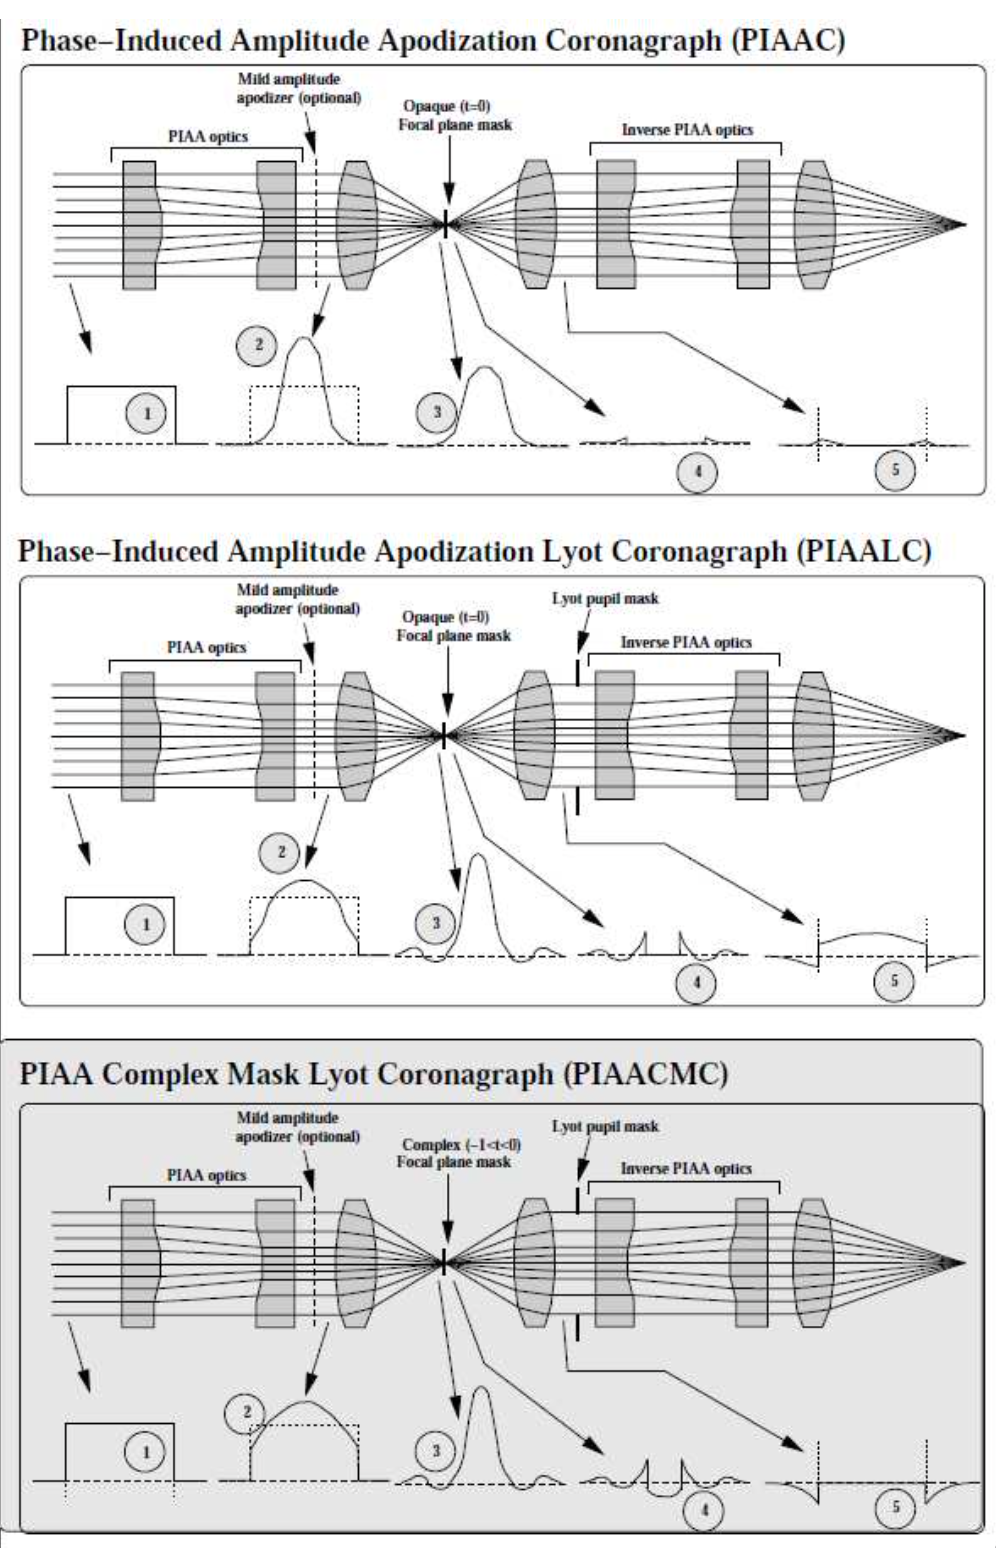
\includegraphics[width=0.5\linewidth]{figures/PIAA_types.png}
  \caption{Different types of PIAA coronagraph. Adapted from Guyon 2011 SPIE paper.}
  \label{fig:piaatypes}
\end{figure}

%The PIAA system approaches the ideal coronagraph limit, making it a compelling choice for small IWA coronagraphs.
%
Original PIAA designs are for unobscured circular apertures: telescope pupils with secondary obscurations require additional formatting of the pupil to make a continuous diffraction-free PSF in the coronagraphic focal plane.
%
The introduction of complex masks that can be manufactured to the required tolerances enable PIAAs for complex and segmented telescope pupils, suitable for space-based telescope designs such as the HabEx/LUVOIR concepts.
%
Results from the laboratory demonstration of a Phase-Induced Amplitude Apodization Complex Mask Coronagraph (PIAACMC) coronagraph with a segmented aperture, \citep{Marx21}, show contrasts of XXXX at YYYY with ZZZZ bandwidth.
%
Most recently, the laboratory demonstration of high contrast with the PIAACMC coronagraph on an obstructed and segmented aperture \citep{Belikov22} shows YYYY contrast achieved.

Ultimately the rejected light can form the basis for a wavefront sensor to keep the PIAA pointed and aligned with the science target, and an integrated WFS and coronagraph with PIAACMC has been demonstrated \citep{Haffert23a}.

\notebooksuggestion{Figure: SH can PIAA simulations for ELT,TMT or GMT (quick!)}

\section{Coronagraphic wavefront sensing}
\lipsum[2-4]

coronagraphic phase diversity
COFFEE jaen paul sauvage 2012 \citep{Sauvage12}.


Gary Ruane 2023 integrated wfs and coronagraphs \citep{Ruane23}

Emiel Por for PAPLC \citep{Por20}

cite Por 2023 or 2021 SPIE Zernike WFS and PAPLC integrated. \citep{Pourcelot22,Pourcelot23}

HiCAT dark zone demonstration \citep{Soummer22}.

SCAR corongaraph using the fiber as a filter \citep{Haffert20}

Direct imaging fiber nulling from \citet{Mawet17} and Eugene Serabyn's paper on fiber nulling from \citet{Serabyn06}.

Using Fresnel zones to make a circular null around the star \citep{Angel86} first time you could detect a Jupiter around a sun-like star.

\todo{Figure: Standard Lyot coronagraph layout}

\todo{Figure: SH: segments, and segment piston errors, impact on dark hole. increase RMS with a slider, then see the dark hole filled in.}

\todo{Figure: ground based coronagraphic images - real would be better, put in SH MagAOX}

\section{Focal plane wavefront sensing}

Imprefections in the manufacture of the optics within a high contrast instrument and the changing environmental conditions result in speckles in the final science camera focal plane.
%
Several techniques for optical sensing of these residual aberrations using telemetry or metrology within the instrument have been partially successful in sensing and removing these aberrations with closed loops, using actively deformable optics to provide correction for the sensed modes.
%
Ultimately, these methods cannot sense the time-varying aberrations within the last optical elements before the science camera focal plane, and so several methods have been developed to measure and characterise optical aberrations using the images from the science camera focal plane.
%
The fundamental challenge is that the vast majority of the science focal plane detectors are photodetectors, and so they do not record the complex amplitude of the incoming electric field in the wavefront, but record only the intensity.

The result is that an intensity image of the PSF cannot be uniquely inverted to give the phase and amplitude of the wavefront in the pupil of the system: an arbitrary wavefront can be represented as the weighted sum of a series of even $f(r)=-f(r)$ and odd $f(r)=-f(-r)$ point symmetric functions.
%
Odd functions produce PSFs with point symmetry (e.g. tip/tilt, coma) but even functions produce the same PSF with the same amplitude but opposite sign - consider a wavefront with focus, which has $\psi(r) = a\sqrt{3}(2r^2-1)$, and both $a$ and $-a$ will result in the same intensity distribution in the focal plane.
%
One of the earliest methods for phase retrieval is therefore an iterative method, the Gerchberg-Saxton algorithm \citep{Gerchberg72}.
%
In this method, an estimate of the pupil plane phase is made by inverse Fourier transforming the PSF and applying the (incorrect) recovered phase in the pupil plane via a deformable mirror or some other active optic.
%
The resultant science camera PSF will be closer to the ideal PSF, and so this loop is repeated until it converges to a flat wavefront - this can be a time consuming process requiring many iterations to get to the required precision.
%
A more rapid optimisation can be made by making informed guesses on the applied phase aberrations\citep{Gonsalves02}, and one such method is the ``fast and furious'' algorithm \citep{Keller12} that has been verified in lab \citep{Wilby18} demonstrated on-sky \citep{Bos20} on ScEXAO. 

In order to measure the complex amplitude of the PSF without an iterative process, a diversity has to be introduced into the focal plane image, either temporally or spatially.
%
For a single point source, all the light in the focal plane is coherent with respect to the core of the PSF.
%
A deformable element within the instrument can then introduce phase shifts into the pupil image that then change the resultant complex amplitude for each location in the focal plane of the science camera.
%
Each pixel in the focal plane then becomes an intensity interferometer, and if four phase shifts that reasonably sample between $0$ and $2\pi$ radians are introduced into the instrument, then the four recorded PSF intensity images can be fit to give an estimate of the complex amplitude at each location in the focal plane.

Calculating the appropriate phases that will result in an optimal sampling and estimate of the complex amplitude for HCI algorithms was presented with a unified formalism by \citet{Giveon09,Giveon10}, called Electric Field Conjugation (EFC).
%
In these papers it was shown that two pairs of complementary deformable mirror actuations can provide enough phase diversity to measure the complex amplitude across the focal plane out to the spatial sampling of the mirror actuators.



Methods include using separate regions of the focal plane to act as proxies for the behaviour of aberrations within the scientifically relevant field of view (REF REF), 

Perspectives on phase retrieval and phase diversity in astronomy \citet{Gonsalves14}.

A review article on phase diversity and focal plane WFS. \citep{Fienup13}

%???not sure what papers for this: traub 2022/2024 intensity nulling

SPHERE papers:

FIGURE: Potier 2022 see Figure~\ref{fig:fpwfsclean} but SH has done it, can do a QSS at 900nm. working to shorter wavelengths

\begin{figure}[ht]
  \centering
  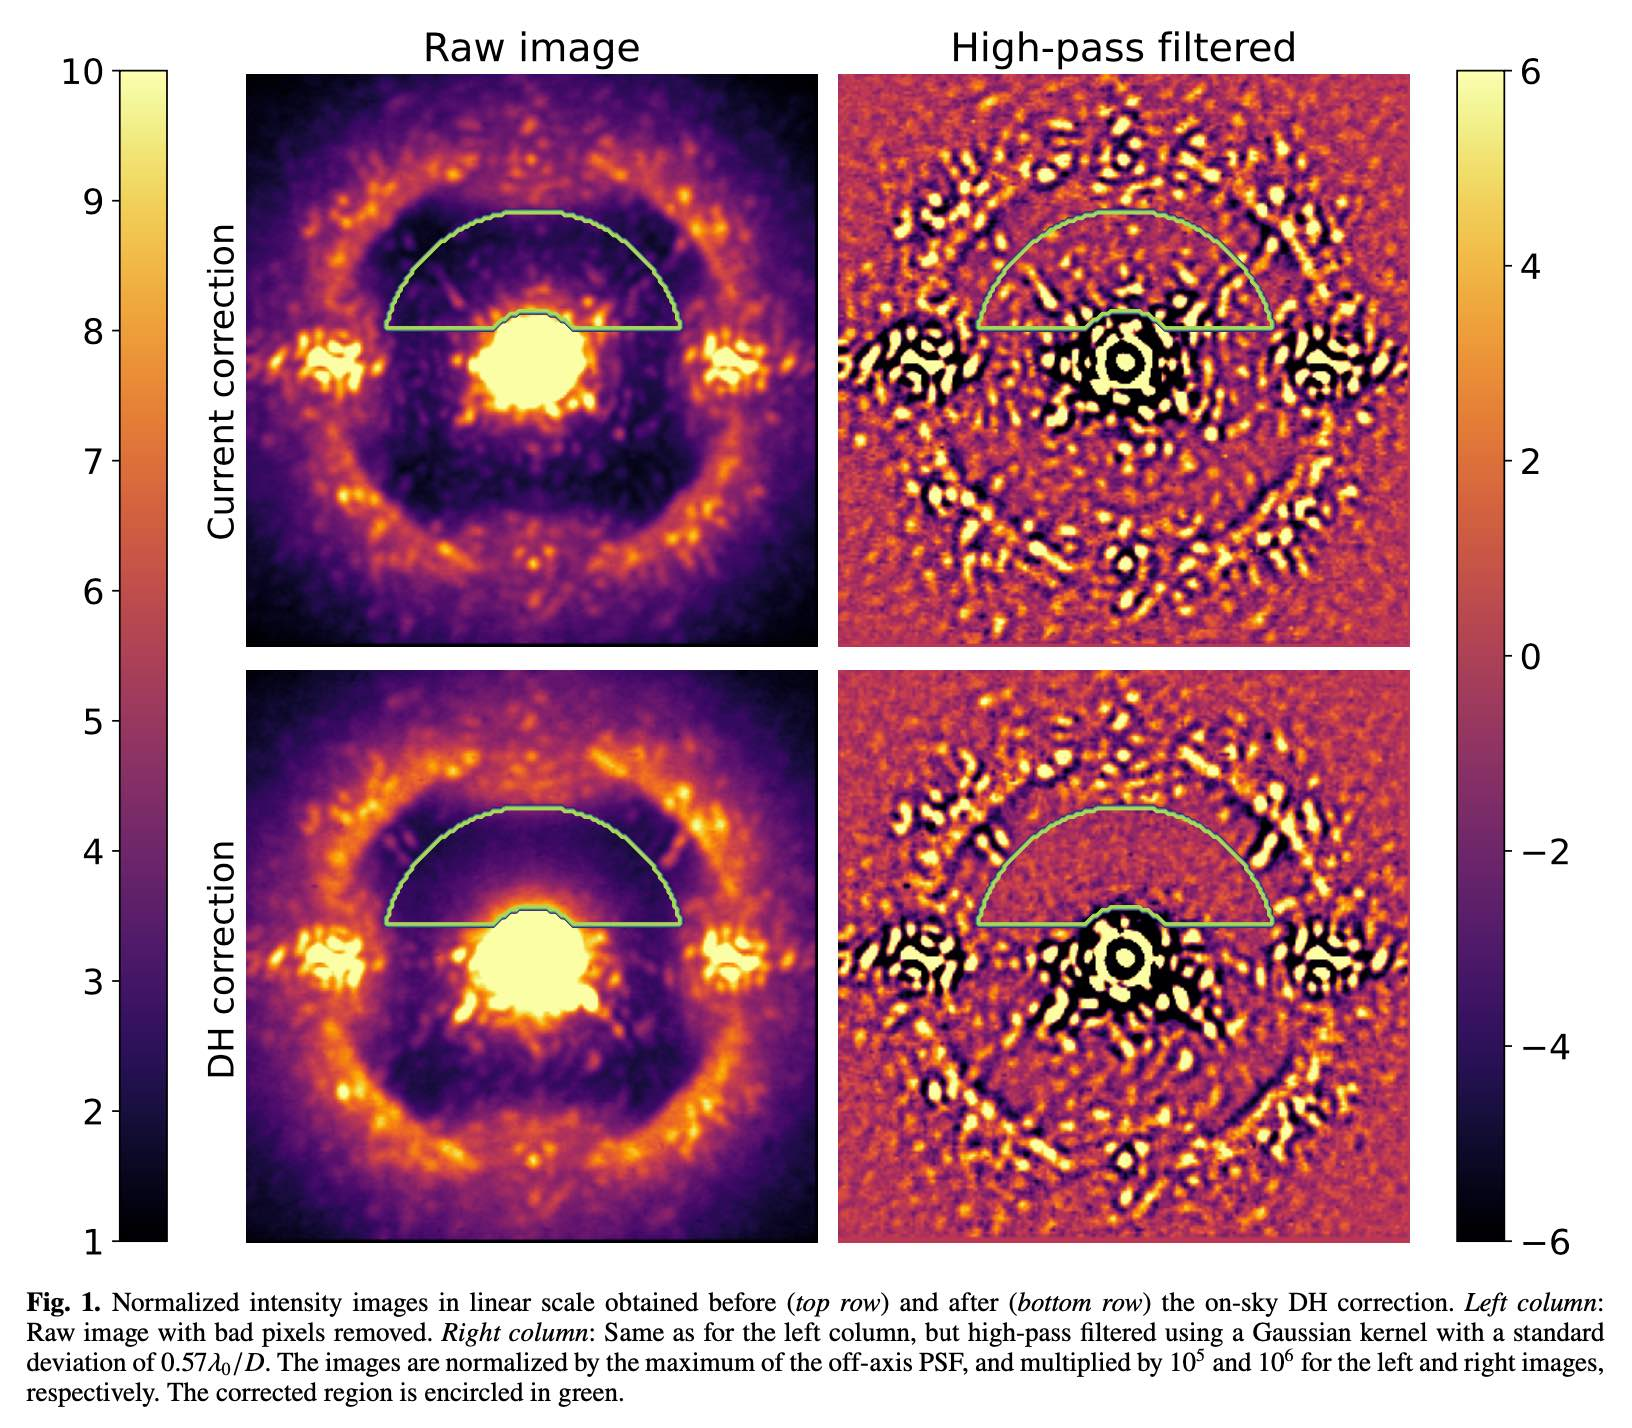
\includegraphics[width=0.6\linewidth]{figures/potier2022.jpg}
  \caption{}
  \label{fig:fpwfsclean}
\end{figure}

\notebooksuggestion{SH: get this from HCIpy Simple dark hole generation with predefined shapes - can use the new autodiff approach.}

\lipsum[2-4]

\section{Rejected light wavefront sensing} 

Visible extreme AO on ELTs for Prox b: \citep{Fowler23}

PAPLC type WFS....

Integrated WFS from Ruane \citep{Ruane20}.

Talk about FAST SCC from Ben Gerard that used rejected light from coronagraph \citep{Gerard18}.


Lyot low order WFS described in \citet{Guyon09} and explored in \citet{Singh14,Singh15}.

%MagAOX paper.... Mcleod et al. 2023

\lipsum[2-4]

\section{PAPLC}

\citet{Por20} 
%Emiel came up with concept, 2019, has unpub paper and SPIE talk...

Haffert 2023 paper

SCOOB 2021 AZ space test bed \citep{Ashcraft22} using a knife edgs SPIE proceeding. PAPLC. \citep{vanGorkom22}.

Figure: SH show unpublished on sky results with PAPLC.

\section{Segmented mirrors}

Larger telescopes are required to increase the spatial resolution of the imaging camera. The cost of a telescope goes as $D^{1.7-1.8}$ \citep{Stahl20} for both, and for space only there is \citet{Stahl10}.
 
Monolithic mirror telescopes are ultimately limited by their transport from manufacturing point to the observatory location, and so segmented telescope designs are used for diameters greater than 8m on the ground.
 %
 Segmented mirror designs are necessary for space telescopes so that the primary mirror can be folded into the faring of rockets.

These segmented mirror designs use active controls and mechanical adjustments to align the mirrors onto the ideal primary mirror surface.
%
This makes segmented mirror designs susceptible to temporal drifts in their alignment, leading to the generation of aberrations in the focal plane that are in the scientific region of interest.

Wavefront sensing and subsequent correction of these aberrations is therefore an important part of high contrast imaging.
%
Algorithms such as COFFEE have been demonstratred for the JWST segmented primary pupil geometry \citep{Leboulleux20}.

Lucie has two papers on redundant apodization for DI of exoplanets - paper I is \citep{Leboulleux22} and paper II is \citet{Leboulleux22a}.

Wavefront tolerances of space-based segmented telescopes at very high contrast: Experimental validation by \citet{Laginja22}

A discussion of the latest limits reached by laboratory coronagraphs is in \citet{Mennesson24}.



HDFS on the GMT is described by \citet{Haffert22}.

Hedglen 2022 Exp valid of piston control with pyramid WFS is in \citet{Bertrou-Cantou23} with the A and A paper detailing it in Confusion in differential piston measurement with the pyramid wavefront sensor \citep{Bertrou-Cantou22}.

GMT: GMT segmented wavefront control Quiros-Pacheco SPIE phaseing for GMT \citep{Quiros-Pacheco22}

% Kautz 2024 in prep. showing on-sky phasing. XX MAK: tried to find this, nothing more recent that 2023

ELT: MELT test bed ZEUS experiment, APE experiment, both phasing experiments form ELT early/mid 2004-2006.

The MELT testbed. MELT: an optomechanical emulation testbench for ELT wavefront control and phasing strategy \citep{Pfrommer18}

ZEUS: a cophasing sensor based on the Zernike phase contrast method: \citep{Dohlen06}.

On-sky Testing of the Active Phasing Experiment  \citet{Gonte09}.

{\bf Keck telescope}

Keck phasing: The original phasing algorithm for Keck mirror segments in \citet{Chanan98} and the second paper in \citet{Chanan00}.

Keck mirror phasing with ZWFS in \citet{vanKooten22} and using a Vector ZWFS in \citet{Salama24}.

On-sky verification of Fast and Furious focal-plane wavefront sensing: Moving forward toward controlling the island effect at Subaru/SCExAO with \citet{Bos20}.

{\bf petal mode problem}

MAK TODO:

LOW WIND EFFECT on SPHERE \citep{Sauvage16} and discussions on mitigating it are described in \citet{Milli18}.

You can use fast and furious to measure it \citep{Wilby18} which was verified at Subaru/SCExAO.

Several mitigation strategies there with FPWFS for that \citep{Vievard19}.

Petal mode problem for ELT: due to the spiders, they fragment the pupil into unsensed separate petals because the thickness of the secondary support is greater than r0.

Even monolithic mirrors have this problem too with thick enough secondary support structures, known as the island effect \citep{Leboulleux22,Leboulleux22a}

\section{Integrated optics}

Optics change the complex amplitudes of wavefronts as they propagate through coronagraphs.
%
Macro optics, typically many thousands of times larger than the wavelength of light they shape, require precise and stable optomechanical components to accurately modify these wavefronts.
%
Integrated optics enable direct manipulation of the complex electric fields at the scale of the wavelengths used.
%
Miniaturisation of previously discrete macro optics and their manufacture within a single homogeneous substrate removes both the requirement for separate optomechanical alignment and temperature related effects.
%

Beam combiners that are required for optical and NIR interferometers require temperature and vibration controlled optical tables with sub-wavelength stability tolerances and alignment for the beamsplitters and associated optics.
%
Manufacture of waveguides within optical materials that perform the beam division and combination considerably simplify the optomechanical requirements, but then the challenges are in coupling the light from the macro optics into the substrates whilst keeping the transmitted efficiency high: diffraction limited optics are required to form PSFs that couple efficiently into the near-single mode sized microoptics.
%
Early examples include beam combiners for optical astronomical interferometers \citep[for example the IOTA/IONIC beam combiner; ][]{Berger01} and photonic lanterns, see \citet{Leon-Saval10} and references therein.
%
Typical coupling efficiencies are on the order of 10\%, increasing to 90\% for more recent designs.

Advances in industry and the requirement for increasingly complex and denser signal transmission lines from the telecommunications industries have made more complex designs realisable for astronomical optics.
%
The optical designs are considerably more challenging, since geometrical optic limits are not a valid approximation.
%
Full electromagnetic propogation is required to design and evalute these microoptic systems, but their complexity also enables new types of optical interactions; devices equivalent to Fabry-Perot etalons can be constructed by etching an elongated loop with one half of the loop parallel to the waveguide - frustrated transmission between the waveguide and the closed loop is modulated as a function of the number of integer wavelengths around the closed loop (REF REF REF).
%https://pure.uhi.ac.uk/en/publications/an-integrated-optics-3-way-beam-combiner-for-iota (REF) 

PIMMS: photonic integrated multimode microspectrograph from \citet{Bland-Hawthorn10}.

Barnaby Norris photonic lanterns \citep{Norris22} and on-sky demo \citep{Norris20} and nature one \cite{Norris20a}, FPWFS with photonic lanterns \citep{Lin20} and their theory \citep{Lin22}.

Nulling with a mode selective photonic lantern 2022 \citep{Xin22}.

Efficient injection from large telescopes into single-mode fibres: Enabling the era of ultra-precision astronomy \citep{Jovanovic17}

Photonic optimised coronagraphs and Integrated photonic-based coronagraphic systems for future space telescopes
 \citep{Desai23a}.

%% Emiel - presented at SPIE 2024 on integrated coronagraphs and photonics - NOTE ONLINE YET.

Bragg gratings to get modulate diffraction \citep{FaggingerAuer24}.

Phase-apodized-pupil Lyot Coronagraphs for Arbitrary Telescope Pupils \citep{Por20}

SCAR paper I \citep{Por20a}

\section{Quantum optimal detection}

Quantum optical detection \citep{Lu18} enables the distinction between two incoherent point sources within the classical Rayleigh diffraction limit.
%
This can be done by a specific linear optic reformatting of the wavefront followed by a photon counting detector.
%
More specifically, for exoplanet detection where the separation is smaller than the diffraction limit and the flux ratio much smaller than one, for thermalised incoherent sources (e.g. a star and a planet) you test for photons not being distributed in a point symmetric way \citep[e.g. ][]{Huang21}.

\citet{Desai23} on deriving this for Achieving Quantum Limits of Exoplanet Detection and Localization.

\section{Post-processing (its no longer a photon)}

\notebooksuggestion{KLIP with removing varying number of modes and annular rings.}

Deviations from the ideal optical prescription of telescope and instrument optics result in wavefront errors which manifest themselves as intensity deviations from the theoretical PSF.
%
Hubble Space Telescope (HST) images of circumstellar material showed residual speckles that obscure the faint circumstellar environment, even after the subtraction of an image of a nearby star used as a reference PSF.

The concept of ``roll subtraction''  \citep{Schneider98} was used to estimate and remove these residual speckles.
%
Two or more images of the science target were taken with the telescope set at different angles about the target axis, so that the astronomical field would be rotated with respect to the (almost static) speckle field.
%
This was demonstrated in \citet{Schneider99} with the image of the disk around HR~4796A.
%
Even with the HST, the roll observations were taken within 25 minutes of each other to minimise changes in the telescope's optical path resulting from the ``breathing'' of the telescope optical assembly as it passed from day to night in its low earth orbit \citep{Bely93}.

With a ground based telescope, the speckle field changes on shorter timescales and with increased complexity because of (i) a continuously changing gravity vector on the telescope and instrument (ii) temperature and mechanical variations in the optomechanics within the instrument and (iii) changes in the performance of the adaptive optics system due to changing atmospheric conditions.

For ground based observations, the concept of Angular Differential Imaging \citep[ADI; ][]{Marois06} was developed.

% this is really spectral methanated differential imaging!
The PSF of ground based time averaged images taken through atmospheric turbulence can be approximated as the telescope PSF with a smoothed Gaussian halo \citep{Marois00}.
%
Methanated camera is called TRIDENT \citep{Marois05}.

Dual band imaging/mathane imaging Beth but also french guy before..., halpha imaging Laird C

This was generalised into Spectral Differential Imaging with SINFONI - thatte 0?
\citet{Thatte07}

Demonstrated with the detection of winds in the atmosphere of HD~209458b \citep{Snellen10} and then molecule mapping in directly imaged exoplanets such as Beta~Pictoris~b \citep{Hoeijmakers18}
High resolution SDI/molecule mapping, Snellen, really high

Polarization differential Imaging \citep{Gledhill91}.

Coherence Differential Imaging: with MKIDS and Ben Mazin VAMPIRES, done it on SPHERE.
Gladyz paper. Remove QSS. Codona, Codona and Kenworthy 2015 (hah!).

Figure: show example of post processing. pick favourite image from a paper!

\lipsum[2-4]

%Disclosure
\section*{DISCLOSURE STATEMENT}
The authors are not aware of any affiliations, memberships, funding, or financial holdings that
might be perceived as affecting the objectivity of this review.

% Acknowledgements
\section*{ACKNOWLEDGMENTS}
M.\ A.\ K.\ acknowledges useful conversations with
Phil Hinz.
% Eric Agol,
% Will Farr,
% Alex Gagliano,
% Tyler Gordon,
% and Maximiliano Isi.

% The authors would like to thank the community members who sent feedback on the public draft of this review:

To achieve the scientific results presented in this article we made use of the \emph{Python} programming language\footnote{Python Software Foundation, \url{https://www.python.org/}}, especially the \emph{SciPy} \citep{virtanen2020}, \emph{NumPy} \citep{numpy}, \emph{Matplotlib} \citep{Matplotlib}, \emph{emcee} \citep{foreman-mackey2013}, and \emph{astropy} \citep{astropy_1,astropy_2} packages.
%

This research has made use of NASA's Astrophysics Data System Bibliographic Services.

% References

\bibliographystyle{ar-style2}
\bibliography{bib}

% \section*{RELATED RESOURCES}

\end{document}
